\newpage
\chapter{Zdroj elektronů, ES40-PS}

Z důvodů problémů s nedostatkem elektronů z wolframového vlákna žárovky jsme se rozhodli k použití ES40-PS jako zdroje elektronů. ES40-PS je \textit{Electron Source Power Supply} poskytující svazek elektronů s nastavitelnou energií, hustotou, pozicí a profilem svazku. Dále umožňuje skenování oblasti s nastavitelnou rychlostí skenování. 


Schéma zapojení zdroje elektronů ES40-PS je znázorněno na Obr.~\ref{04schema} vlevo. Zdroj elektronů je upevněn pomocí průchodky do vakuové komory a připojen ke stanici ES40-PS pomocí kabelu s 6-pinovou spojkou. Na Obr.~\ref{04schema} vpravo je zobrazena ukázka ovládacího panelu stanice ES40-PS. 


\begin{figure}[htbp!]
\centering
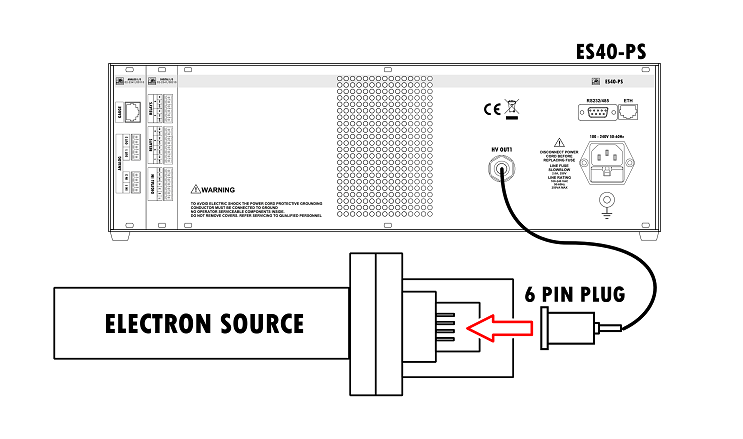
\includegraphics[width = 170 pt]{Figure/04/schema.png}
\hfill
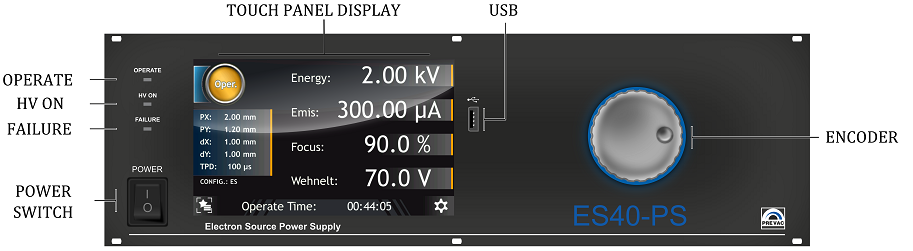
\includegraphics[width = 250 pt]{Figure/04/panel.png}
\caption[Schéma zapojení a ukázka ovládacího panelu stanice ES40-PS]{Vlevo: Schéma zapojení zdroje elektronů ES40-PS. Vpravo: Ukázka předního ovládacího panelu stanice ES40-PS. Převzato z~\cite{Manual}.}
\label{04schema}
\end{figure}

Zdroje elektronů ES40-PS má několik nastavitelných parametrů: 
\begin{itemize}
\item \textbf{Urychlovací napětí} je nastavitelné od 0 kV do 5 kV
\item \textbf{Emisní proud} elektronů je nastavitelný v rozmezí od $0{,}01 \ \mu$A do $300{,}00 \ \mu$A
\item \textbf{Fokusovací napětí} je spojené s urychlovacím a lze nastavit od 60,0 \% do 99,9 \%
\item \textbf{Wehneltovo napětí} od 0 V do 300 V
\end{itemize}
Elektrony vychází ze zahřívání wolframové katody, z tohoto důvodu se může objevit zpráva "Current Limit", kdy je zapotřebí více času ke stabilizaci emisního proudu. 

Zmíněné hodnoty je možné nastavit na úvodní obrazovce ovládacího panelu viz Obr.~\ref{04display}. Po kliknutí na zmenšený seznam hodnot nacházející se v levé části se display přepne do druhé polohy, kde je možné nastavit následující hodnoty:
\begin{itemize}
\item \textbf{Horizontální výchylka} PX je nastavitelná v rozmezí od $-5{,}00$ mm do $5{,}00$ mm 
\item \textbf{Vertikální výchylka} PY je nastavitelná v rozmezí od $-5{,}00$ mm do $5{,}00$ mm 
\item \textbf{Horizontální rozsah skenu} dX je nastavitelný v rozmezí od $0{,}00$ mm do $10{,}00$ mm
\item \textbf{Vertikální rozsah skenu} dY je nastavitelný v rozmezí od $0{,}00$ mm do $10{,}00$ mm
\item \textbf{TPD hodnota} (\textit{time per dot}) je nastavitelný v rozmezí od $20 \ \mu$s  do $30$ ms
\end{itemize}
Při současném nastavení výchylky a skenu se může objevit zpráva "SCAN X/Y OVERFLOW", která značí překročení fyzikálního rozsahu zdroje elektronů ES40-PS a pro její odstranění je nutné snížit výchylku svazku nebo rozsah skenování. 

\begin{figure}[htbp!]
\centering
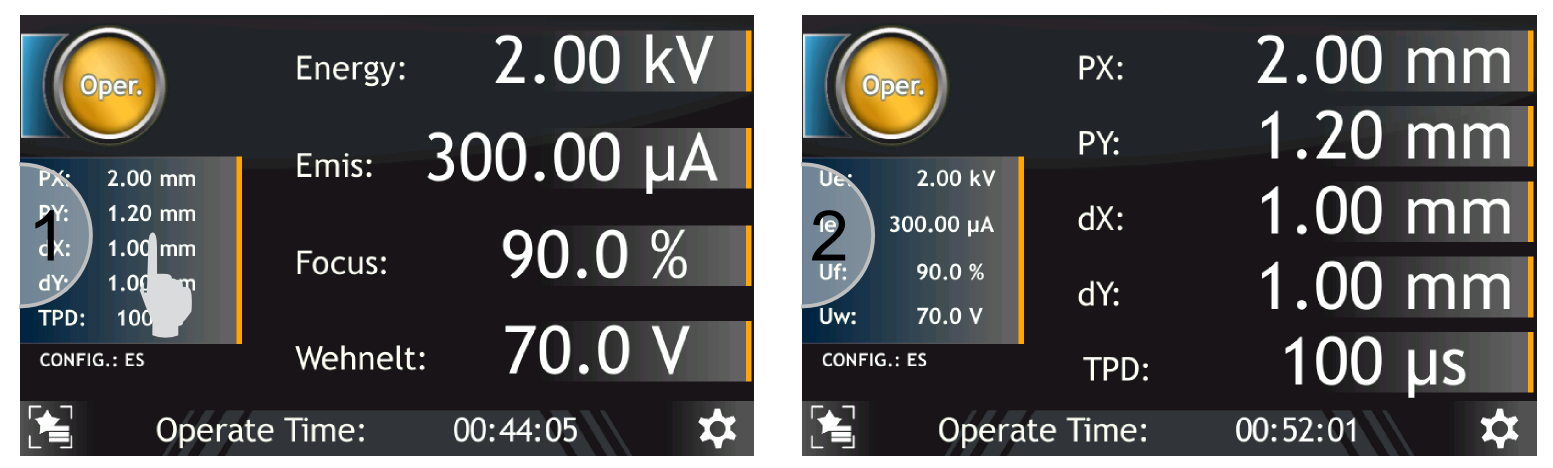
\includegraphics[width = 370 pt]{Figure/04/display.png}
\caption[Ukázka nastavení parametrů zdroje elektronů]{Ukázka nastavení parametrů zdroje elektronů a přepnutí do druhého menu. Převzato z~\cite{Manual}}
\label{04display}
\end{figure}

%princip změny polohy?
%
%\begin{figure}[htbp!]
%\centering
%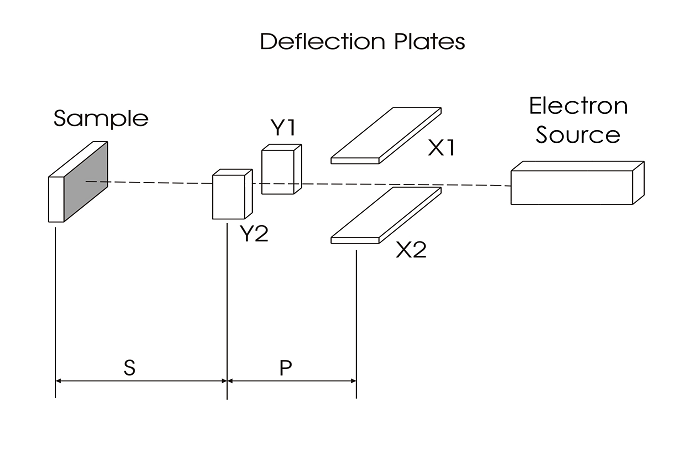
\includegraphics[width = 170 pt]{Figure/04/schema2.png}
%\caption{. Převzato z~\cite{Manual}}
%\label{04schema2}
%\end{figure}

Spuštění zdroje elektronů ES40-PS krok za krokem:
\begin{enumerate}
\item Po zapnutí napájení by měl být zdroj ponechán v režimu \textit{STAND-BY} alespoň 10 minut pro řádné zahřátí a stabilizaci katody
\item Pokud zdroj nebyl použit delší dobu následuje \textit{DEGAS} procedura
\item Následuje zapnutí do \textit{OPERATE} módu, ale pouze v případě je-li tlak v komoře nižší než $5 \times 10^{-6}$ mbar
\item Doporučené začínající hodnoty jsou: Energie = 3 kV, Emise = 100 $\mu$A, Fokusace = 70 \%, Wehneltovo napětí = 85 V, PX = PY = dX = dY = 0 mm
\end{enumerate} 


\textbf{DEGAS} procedura
\begin{enumerate}
\item Před zapnutím do \textit{OPERATE} módu je nutné nastavit všechny napětí a proudy na minimum. 
\item Po zapnutí do \textit{OPERATE} módu je nutné nastavit následující parametry v daném pořadí: Energie = $2{,}00$ kV, Fokusace = $88{,}0$ \% a Wehneltovo napětí = $71{,}0$ V
\item Zvýšení Emise na $300{,}00 \ \mu$A 
\item S tímto nastavením by mělo zařízení pracovat 10 minut
\item Následně by měla být emise snížena na minimum a poté i zbývající napětí
\end{enumerate}
Během \textit{DEGAS} procedury by měly být parametry zvyšovány postupně se současnou kontrolou tlaku v komoře. Pokud dojde k náhlému poklesu vakua v komoře, mělo by být zařízení ponecháno se stávajícími parametry dokud nedojde k obnovení vakua.

Více podrobností k ovládání zdroje elektronů ES40-PS je popsáno v operačním manuálu ~\cite{Manual}.